\chapter{Graph-Datenbanken - Grundlegende technologische Aspekte}
\section{Modell}
Allgemein betrachtet ist ein Modell eine vereinfachte bzw. abstrahierte Darstellung von realen Gegenständen, Sachverhalten oder Problemen.
Durch die Modellierung soll die Realität auf die wichtigsten Einflussfaktoren reduziert werden \cite{datamodels}.
In der Datenbankwelt beschreibt das Modell die Struktur der Daten, Operationen zum manipulieren der Daten und Integritätsbedingungen \cite{efcodd}.
Das derzeit am häufigsten verwendete Modell ist das relationale Datenbankmodell, bei dem die Daten in Tabellen gespeichert werden und in der Regel die standardisierte Abfragesprache \ac{SQL} eingesetzt wird.
Der Schwachpunkt des relationalen Datenbankmodells liegt bei der Verarbeitung von Daten mit einer hohen Anzahl an Beziehungen \cite{vicknair2010comparison}.

%Die Graphentheorie spielt eine zentrale Rolle bei der Modellierung, da sich Graphen sehr gut zur Darstellung vernetzter Daten eignen.
Da eine effiziente Verarbeitung von großen vernetzten Datenmengen immer wichtiger wird, haben Graphenmodelle in den letzten Jahren im Datenbankbereich stark an Bedeutung gewonnen.
Graph-Datenbanken nutzen Graphen als Datenbankmodell und greifen auf graphenspezifische Operationen zur effizienten Verarbeitung vernetzter Daten zurück \cite{angles2008survey}.
%Obwohl sich die verschiedenen Graphdatenbanken im allgemeinen nur minimal bei der Strukturierung der Daten unterscheiden, gibt es sehr verschiedene Ansätze bei den Abfragesprachen \cite{anglesintro}.
%Dennoch sind die kleinen Unterschiede in der Datenmodellierung oft entscheidend und es können je nach Anwendungsfall verschiedene Modelle sinnvoll sein \cite{angles2012comparison}.
Trotz der oft kleinen Unterschiede in der Datenmodellierung können je nach Anwendungsfall verschiedene Modelle sinnvoll sein \cite{angles2012comparison}.
In der Praxis werden oft verschiedene Modelle zu Multi-Model Datenbanken kombiniert, um die Schwachpunkte der einzelnen Modelle auszugleichen.
Ein Beispiel für eine solche Multi-Model Datenbank ist OrientDB, welche unteranderem das Graphen-Modell mit Key-Value Stores und dem Objektorientierten-Modell verbindet \cite{orient}.
Im folgenden sollen verschiedene Graphdatenbankmodelle, sowie Aspekte der Graphentheorie, die zur Modellierung von Graphdatenbanken von Bedeutung sind, kurz vorgestellt werden.
\newpage
\subsection{Graph}
%Ein Graph G besteht aus einer nichtleeren Menge an Knoten V und Kanten E.
%Ein Graph ist mathematisch folgendermaßen definiert:
Die Grundlage aller Graphdatenbankmodelle liefert die Definition eines einfachen Graphen:
\begin{definition}
	Ein $\text{Graph } G=(V,E,\gamma)$ ist ein Tripel bestehend aus:
	\begin{itemize}
		\item $V$, einer nicht leeren, ungeordneten Menge von Knoten (vertices)
		\item $E$, einer Menge von Kanten (edges)
		\item $\gamma$ , einer Inzidenzabbildung (incidence relation), mit\\
		$\gamma : E \longrightarrow \{X | X \subseteq V, 1 \leq |X| \leq 2\}$
	\end{itemize}\cite[Seite 21]{pbeck01}
%	Ein Knoten $a \in V$ und eine Kante $e \in E$ heißen inzident (incident)
%	genau dann wenn $a$ entweder Anfangs- oder Endecke von $e$ ist. Es gilt $a \in \gamma(e)$.
%	Zwei Knoten $a,b \in V$ heißen adjazent(adjacent) genau dann wenn es eine Kante $e$ gibt die zu $a$ und $b$ inzident ist.
%	Es gilt	$\exists e \in E: \gamma(e)=\{a,b\}$.
\end{definition}
Ein Knoten representiert ein Element in einem Graphen und die Kanten stellen die Beziehung zwischen den einzelnen Knoten her.
%In einem einfachen Graphen kann eine Kante immer nur jeweils zwei Knoten miteinander verbinden.
Bei einfachen Graphen können die Kanten nur die Kardinalität $1 \leq |X| \leq 2$ haben.
Als Kardinalität wird die Anzahl Knoten bezeichnet, die durch eine Kante in Beziehung gesetzt werden kann.
Zwei Knoten heißen adjazent, wenn diese über eine Kante direkt miteinander verbunden sind.
Eine Kante die mit einem Knoten verbunden ist wird als inzident zu diesem Knoten bezeichnet \cite{knauer2015diskrete}.

%\subsection{Eigenschaften von Kanten}
Graphen können gerichtet oder ungerichtet sein.
Gerichtete Graphen zeichnen sich dardurch aus, dass die Kanten eine zugewiesene Richtung besitzen.
Grafisch werden gerichtete Kanten in der Regel durch Pfeile dargestellt.
Für die Modellierung von realen Gegebenheiten ist das Konzept der gerichteten Graphen sehr entscheidend, da dieses die Darstellung einseitiger Beziehungen zwischen den Entitäten des Modells erlaubt.

Um die Beziehung zwischen zwei Knoten genauer zu definieren, lassen sich die Kanten gewichten.
Dabei werden den Kanten in der Regel nummerische Werte zugeordnet und man bezeichnet diese Graphen als gewichtete Graphen.
Durch die Wichtung von Kanten lassen sich beispielsweise Kosten oder Distanzen zwischen den Entitäten definieren.

Ein Knoten ist isoliert, wenn er keine inzidenten Kanten und somit keine direkten Nachbarn hat \cite{knauer2015diskrete}.
Ein ungerichteter Graph heißt zusammenhängend, falls es zwischen zwei beliebigen Knoten $a$ und $b$ aus $V$ einen ungerichteten Weg mit $a$ als Startknoten und $b$ als Endknoten gibt \cite[36-38]{krumke2012graphentheoretische}.
Hat eine Kante als Start- und Endknoten den selben Knoten, verbindet also den Knoten mit sich selber, spricht man von einer Schlinge.
Liegen zwischen zwei Knoten eines Graphen mehr als eine Kante, nennt man diese Multikante.
Enthält ein Graph Multikanten und Schlingen ist dies kein einfacher Graph mehr sondern ein Multigraph \cite{felsner01}.
%Schlingen und Multikanten dürfen in einem einfachen Graphen nicht auftauchen.\cite{felsner01}

Der Grad eines Knoten bezeichnet die Anzahl der inzidenten Kanten des Knoten.
Dabei werden Schleifen doppelt gezählt \cite{rahm2017}.
Ein Graph, bei dem alle Knoten den selben Knotengrad haben, wird als regulärer Graph bezeichnet \cite{felsner2012geometric}.
%Abbildung \ref{2.regular.image} zeigt einen regulären Graphen mit Knotengrad null und einen mit einem Grad von drei.
%\begin{center}
%	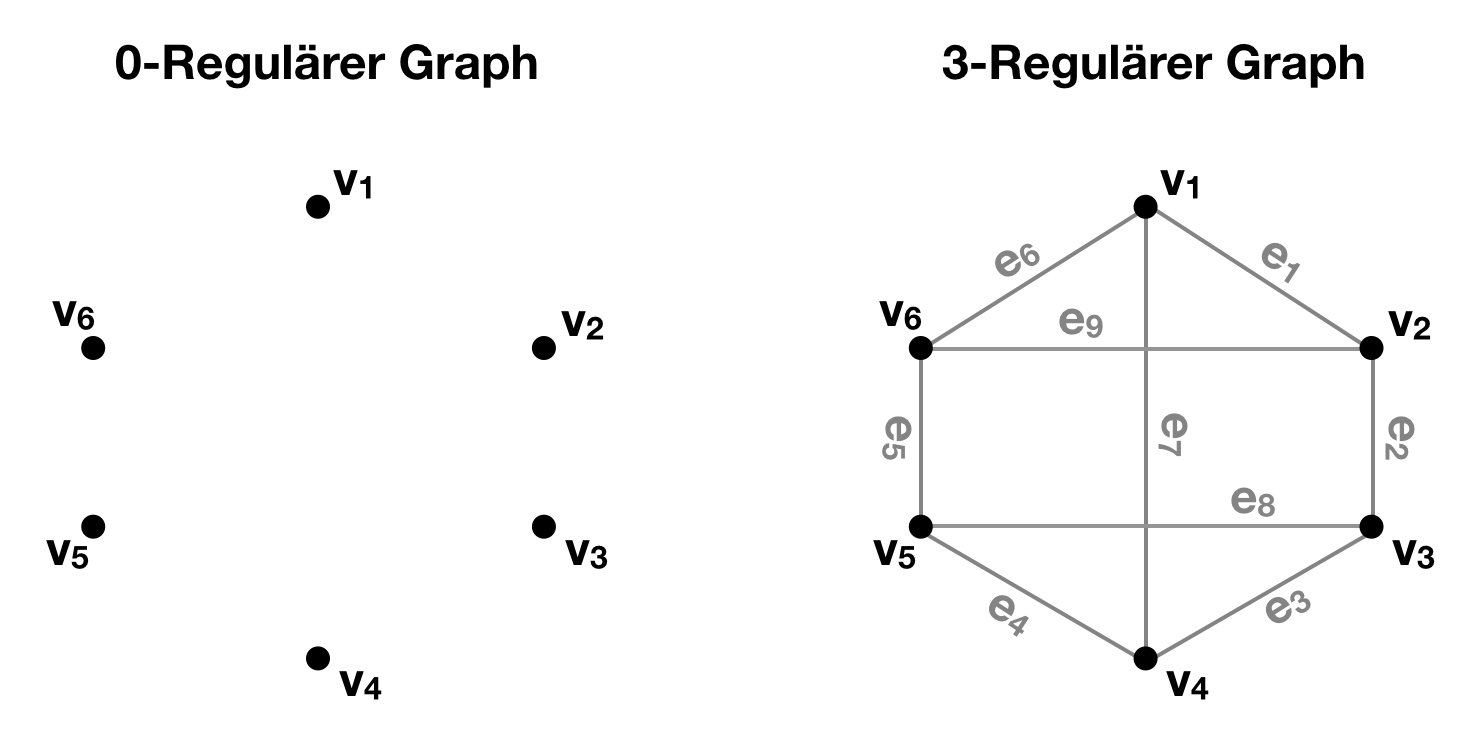
\includegraphics[scale = 0.4]{./images/Regulaerer_graph.png}
%	\label{2.regular.image}
	%\caption{Regulärer Graph}
%\end{center}
Sind bei einem Graphen alle Knoten mit allen übrigen Knoten verbunden, spricht man von einem vollständigen Graphen:
\[K_{n}=\big([n],\begin{pmatrix}
					 [n] \\ 2
\end{pmatrix}\big)\]

%Werden Kanten und Knoten eines Graphs vertauscht, entsteht der Kantengraph bzw. Line-Graph des jeweiligen Graphen L(G).
Da bei einem Graphen nur die Struktur definiert ist, also welcher Knoten über welche Kante mit den anderen Knoten verbunden ist, können Graphen auf unterschiedliche Weisen gezeichnet werden und trotzdem gleich sein.
Sind zwei Graphen gleich, bezeichnet man diese als isomorph \cite[Seite 22]{basicgraphtheory}.
%
%Das simpelste Graphdatenbankmodell ist ein einfacher gelabelter Graph.
%
%Subgraphen
%\subsection{Reguläre Graphen}
%Bei regulären Graphen haben alle Knoten den selben Knotengrad.
%Als Knotengrad wird die Anzahl direkter Nachbarn, also alle Knoten die über eine Kante direkt mit dem betrachteten Knoten verbunden sind, bezeichnet.\cite{felsner2012geometric}
%Abbildung \ref{2.regular.image} zeigt einen regulären Graphen mit Knotengrad null und einen mit einem Grad von drei.
%\begin{center}
%	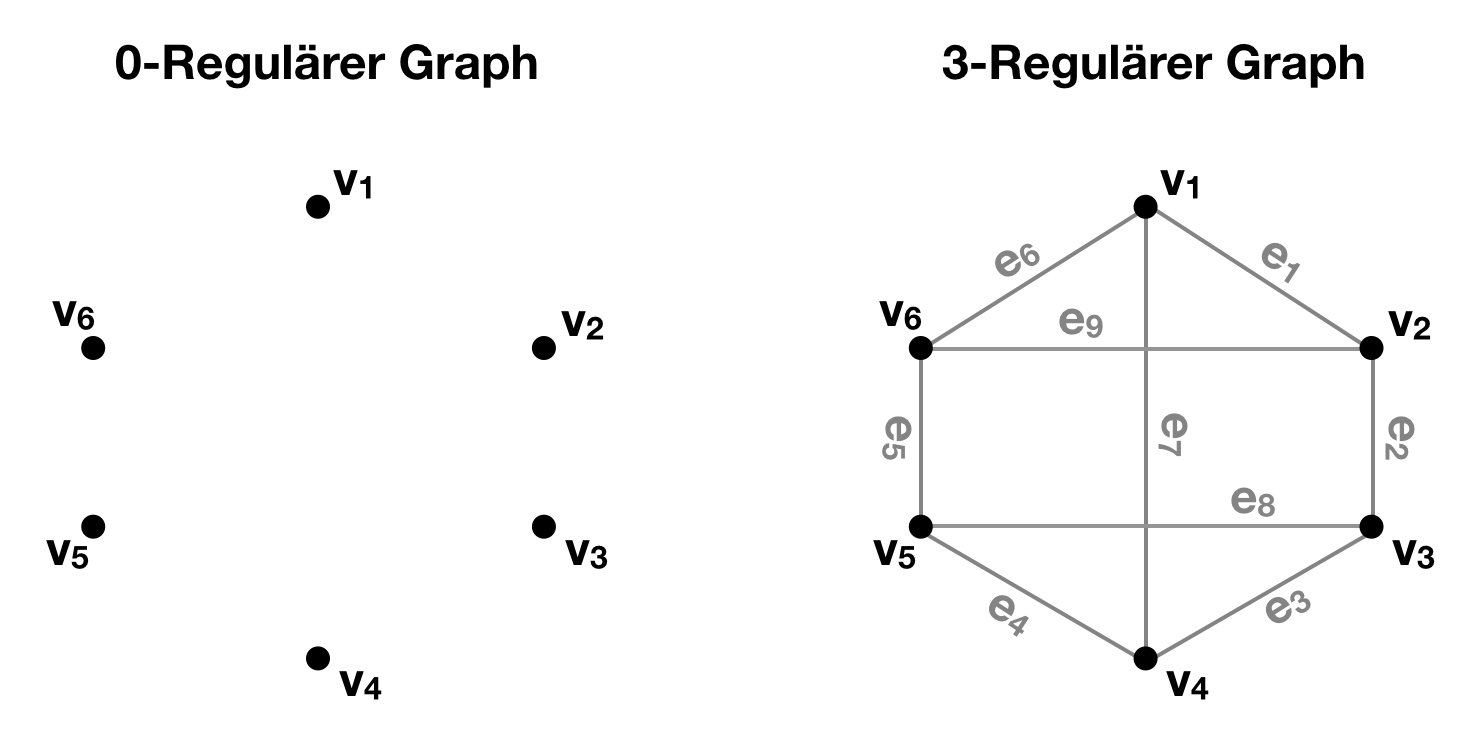
\includegraphics[scale = 0.4]{./images/Regulaerer_graph.png}
%	\label{2.regular.image}
%	%\caption{Regulärer Graph}
%\end{center}
\subsection{Bäume}
Ist ein Graph kreisfrei, es gibt keinen Weg bei dem der Start- gleich dem Endknoten ist, spricht man von einem Wald.
Sind die Knoten eines Waldes zusammenhängend entsteht ein Baum.
%Ein Baum mit $n$ Knoten hat immer $n-1$ Kanten \cite{basicgraphtheory}.
Knoten mit dem Grad $n=1$ werden als Blätter bezeichnet.
Bäume können gerichtet und ungerichtet sein.
Im Falle von gerichteten Bäumen spricht man auch von gewurzelten Bäumen, da der Ursprungsknoten als Wurzel bezeichnet wird.
Abbildung \ref{2.baum.image} zeigt einen gewurzelten Baum, die Blätter sind hier grün dargestellt und die Wurzel rot.
In einem Baum gibt es zwischen zwei beliebigen Knoten immer nur einen Weg \cite{basicgraphtheory}.
%Bei einem gewurzelten Baum werden die Ausgangsknoten als Eltern und die Zielknoten jeweils als Kinder der Ausgangsknoten bezeichnet.
%Hat in einem gewurzelten Baum jeder Knoten maximal zwei Kinder, wird dieser als Binärbaum bezeichnet \cite{basicgraphtheory}.
\begin{figure}[H]
	\begin{center}
	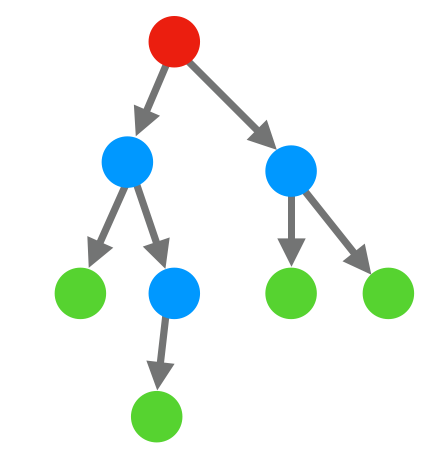
\includegraphics[scale = 0.3]{./images/baum.png}
	\label{2.baum.image}
    \caption{gewurzelter Baum}
	\end{center}
\end{figure}
Bäume sind Grundlage unteranderen des hierarchischen Datenbankmodells, welches sich dadurch auszeichnet, dass jeder Knoten nur einen Vorgänger haben kann.
Dieses Datenbankmodell hat den Nachteil, dass bedingt durch die Kreisfreiheit eines Baumes sehr eingeschränkt ist und beispielsweise keinen:n Beziehungen modelliert werden können.
Das Netzwerkdatenbankmodell versucht dieses Problem zu lösen, indem die Limitierung auf einen Vorfahren aufgehoben wird \cite{hald2013datenbank}.
\subsection{Property Graphen}
Property Graphen erweitern das Modell des einfachen Graphen.
Property Graphen sind gerichtete Graphen, die sich durch ihre den Kanten und Knoten zugewiesenen Eigenschaften (Properties) auszeichnen.
Gespeichert werden diese Eigenschaften als Key-Value-Paare.
Das Hinzufügen von Attributen an einen Knoten oder eine Kante soll zusammengehörige Daten schneller abrufbar machen \cite{angles2012comparison}.
Label ermöglichen die Unterteilung von Knoten und Kanten in verschiedene Knoten- und Kantentypen.
Attribute, Label und die Richtung der Kanten erlauben eine sehr detaillierte Modellierung von realen Sachverhalten.
Somit sind Property Graphen von sehr großer Bedeutung für die Modellierung von Graphdatenbanken.

Abbildung \ref{2.property.image} zeigt einen Property Graphen.
Die Knoten sind den drei Labeln Person, Unternehmen und Stadt zugeordnet.
Die gerichteten Kanten stellen die Beziehungsverhältnisse zwischen den einzelnen Knoten her und können durch Attribute, wie beispielsweise der Information über die Dauer der bisherigen Beziehung, genauer definiert werden.
\begin{figure}[H]
\begin{center}
	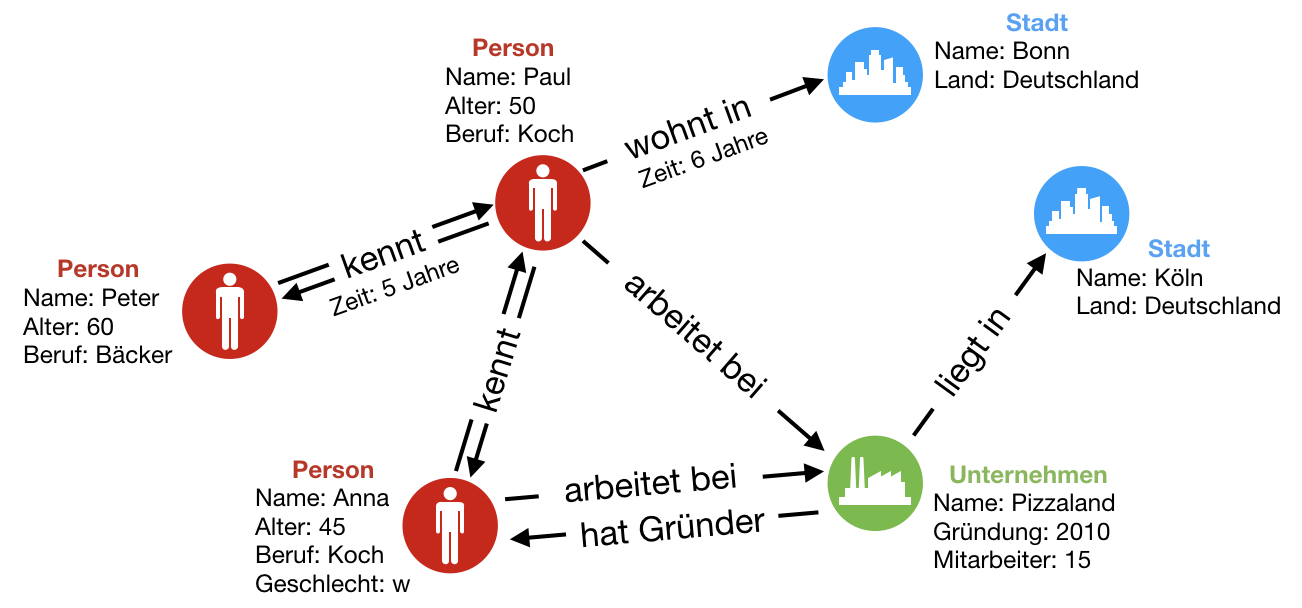
\includegraphics[scale = 0.65]{./images/Property_graph.png}
	\label{2.property.image}
	\caption{Property Graph}
\end{center}
\end{figure}


Der Vorteil von Property Graphen ist, dass diese eine sehr detailierte Modellierung der Daten ermöglichen.
Nachteilig ist, dass eine komplexere Datenstruktur zu einer komplizierteren Realisierung führt.
Derzeit sind Property Graphen das am häufigsten verwendete Datenmodell für Graphdatenbanken.
Neo4j, die momentan weltweit populärste Graphdatenbank, nutzt Property Graphen als Datenbankmodell \cite{neo4j}.
Ein weiteres Beispiel für ein Graph \ac{DBMS}, welches Property Graphen zur Modellierung nutzt, ist JanusGraph \cite{janus}.

\subsection{Hypergraphen}
Hypergraphen stellen eine Generalisierung von Graphen dar und ermöglichen die Modelierung komplexer Beziehungen \cite{anglesintro}.
%Hypergraphen haben die Eigenschaft, dass Kanten im Gegensatz zu klassischen Graphen mehr als zwei Knoten miteinander verbinden können.
%Die Kanten des Hypergraphen werden auch als Hyperkanten bezeichnet.
Im Vergleich zum normalen Graphen können die Kanten eines Hypergraphen eine beliebige Kardinalität haben.
Die Hyperedges in einem Hypergraphen verbinden somit eine beliebige Menge von Knoten, was eine direkte Darstellung von Beziehungen höherer Ordnung ermöglicht \cite{iordanov2010hypergraphdb}.
Im Falle eines gerichteten Hypergraphen verbindet die Hyperkante den Ausgangsknoten direkt mit allen Zielknoten.
%\\Mathematisch ist ein Hypergraph folgendermaßen definiert:
%\begin{definition}
%	Let $X=\{v_{1}, v_{2},...,v_{n}\}$ be a finite set,
%	and let $E=\{e_{1},e_{2},...,e_{m}\}$ be a family of subsets of $X$ such that
%	\[e_{i} \neq \varnothing (i=1,2,...,m) \\
%	\cup_{i=1}^{m}e_{i}=X.
%	\]
%	The pair $H=(X,E)$ is called a hypergraph with vertex set $X$
%	and hyperedge set $E$. The elements $v_{1}, v_{2},...,v_{n}$ of $X$ are vertices
%	of hypergraph $H$, and the sets $e_{1}, e_{2},...,e_{m}$ are hyperedges of hypergraph $H$ \cite[Seite 2]{zhang2018hypergraph}.
%\end{definition}

Abbildung \ref{2.hyper.image} zeigt einen Hypergraphen.
Die Kante $e_{4}$ verbindet in diesem Graphen die Knoten $v_{5}$, $v_{6}$ und $v_{7}$ miteinander.
\begin{figure}[H]
\begin{center}
	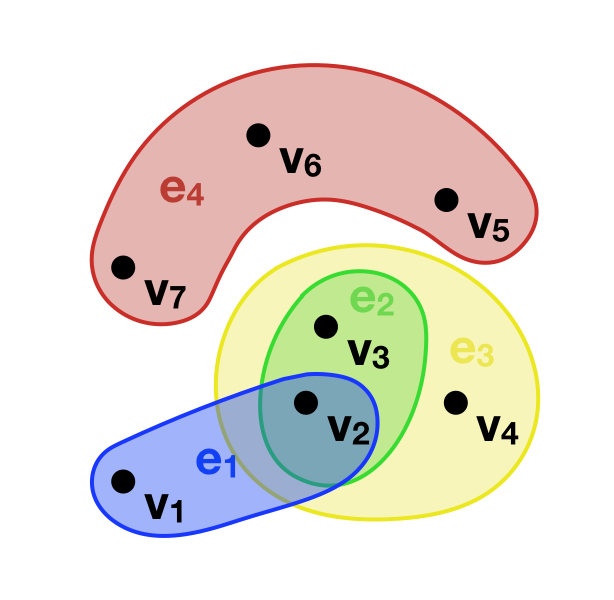
\includegraphics[scale = 0.5]{./images/Hypergraph2.png}
	\label{2.hyper.image}
	\caption{Hypergraph}
\end{center}
\end{figure}
%Hypergraphen ermöglichen die direkte Darstellung rekursiver Beziehungen \cite{iordanov2010hypergraphdb}.
Da Hypergraphen die direkte Darstellung rekursiver Beziehungen ermöglichen und somit eine flexiblere Struktur als das einfache Graphen-Modell bieten, werden diese oft zur Modellierung in Graphdatenbanken verwendet \cite{iordanov2010hypergraphdb}\cite{flockdb}.
Eine Datenbank, die Hypergraphen als Datenbankmodell nutzt ist beispielsweise HyperGraphDB, welche von Kobrix Software Inc entwickelt wurde \cite{iordanov2010hypergraphdb}.
Ein weiteres Projekt, bei dem Hypergraphen zur Modellierung genutzt werden ist Trinity \cite{shao2013trinity}.
%In einem normale Graphen sind die Kanten, eine in einem Intervall festgelegte Menge von Knoten:
%    \[X = \{v_{1}, v_{2}, v_{3}, v_{4}, v_{5}, v_{6}, v_{7}\} \text{ Knoten}\]
%    \[E=\{e_{1}, e_{2}, e_{3}, e_{4}\} \text{ Kanten}\]
%    \[E=\{e_{1}, e_{2}, e_{3}, e_{4}\} = \{\{v_{1}, v_{2}, v_{3}\}, \{v_{2}, v_{3}\}, \{v_{3}, v_{5}, v_{6}\}, \{v_{4}\}\} \]
%Transversals
%\subsection{Multimodale Graphen}
%\subsection{Hypertree}
%\subsection{k-uniform hypergraph}
\subsection{Verschachtelte Graphen}
%Hypernodes ermöglichen die Verschachtelung von Graphen, was bedeutet, dass ein Knoten wiederum ein Graph sein kann
In einem verschachtelten Graphen kann ein Knoten wiederum ein Graph sein. Diese Knoten werden als Hypernodes bezeichnet.
Das Konzept von Hypernodes erlaubt eine beliebig große Komplexität des Modells.
Das Hypernode Modell nutzt gerichtete Kanten.
Jeder Knoten des verschachtelten Graphen bekommt ein eindeutiges Label.
Um die Knoten in verschiedene Kategorien zu unterteilen werden Tags vergeben \cite{poulovassilis1994nested}.

Abbildung \ref{2.hypernode.image} stellt einen Teil des in \ref{2.property.image} dargestellten Property Graphen als Hypernodes dar.
Alle Knoten haben ein eindeutiges Label und es wurden zwei Tags vergeben - Unternehmen und Person.
Durch gerichtete Kanten werden die Beziehungen zwischen den einzelnen Hypernodes hergestellt.
Die Attributer, die im Property Graphen als Key-Value Paare gespeichert werden, werden im verschachtelten Graphen als Knoten einer Hypernode gespeichert.
\begin{figure}[H]
	\begin{center}
		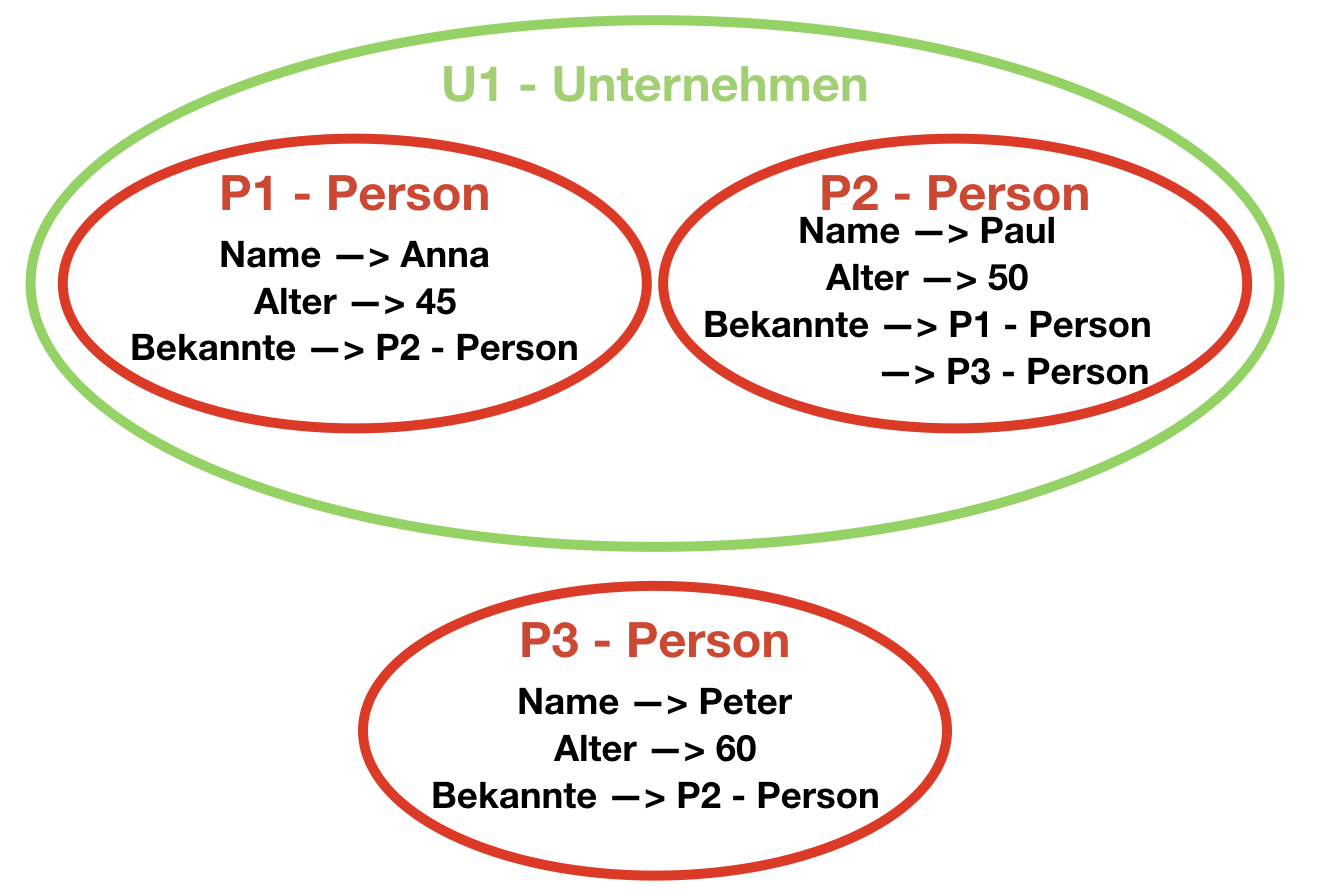
\includegraphics[scale = 0.5]{./images/Hypernode.png}
		\label{2.hypernode.image}
		\caption{Hypernode}
	\end{center}
\end{figure}

Hypergraphen lassen sich durch Hypernodes darstellen, indem man die im Hypergraph durch eine Hyperedge verbundenen Knoten in einer Hypernode modelliert.
Umgekehrt lassen sich Hypernodes nicht unbedingt in einem Hypergraphen realisieren \cite{poulovassilis1994nested}.